\section{Results \& Discussion}\label{sec:results}

\subsection{Fitting Sorption Parameters}

Using the numerical fitting scheme described in section \ref{sec:indoor_environment} with the sorption data from the method described in section \ref{sec:experimental_method}, the kinetic sorption parameters $k_1$ and $k_2$ are fitted.
Figure \ref{fig:sorption_fit} shows the result of this fitting and the sorption data for three select materials - wood, Appling soil, and cinderblock concrete.
The $k_1$ and $k_2$ represent the rate at which TCE desorbs and sorbs respectively onto/from the material of interest.
The equilibrium sorption constant is, using the formulation in \eqref{eq:sorption_rate}, given by
\begin{equation}
  K = \frac{k_1}{k_2}
\end{equation}
and is used as the sorption isotherm.
Here a small $K$ indicate that there is a greater propensity for contaminant sorption.\par

To use the soil sorption isotherm in \eqref{eq:mass_transport} $K$ needs to be converted from being unitless to $\mathrm{m^3/kg}$.
This is done by multiplying the inverse of $K$ isotherm with inverse of the soil bulk density $\rho_b$, which is taken to be $1460 \; \mathrm{kg/m^3}$.
\begin{equation}
  K_\mathrm{ads} = \frac{1}{K \rho_b} = 5.28 \; \mathrm{(m^3/kg)}
\end{equation}

\begin{figure}[htb!]
  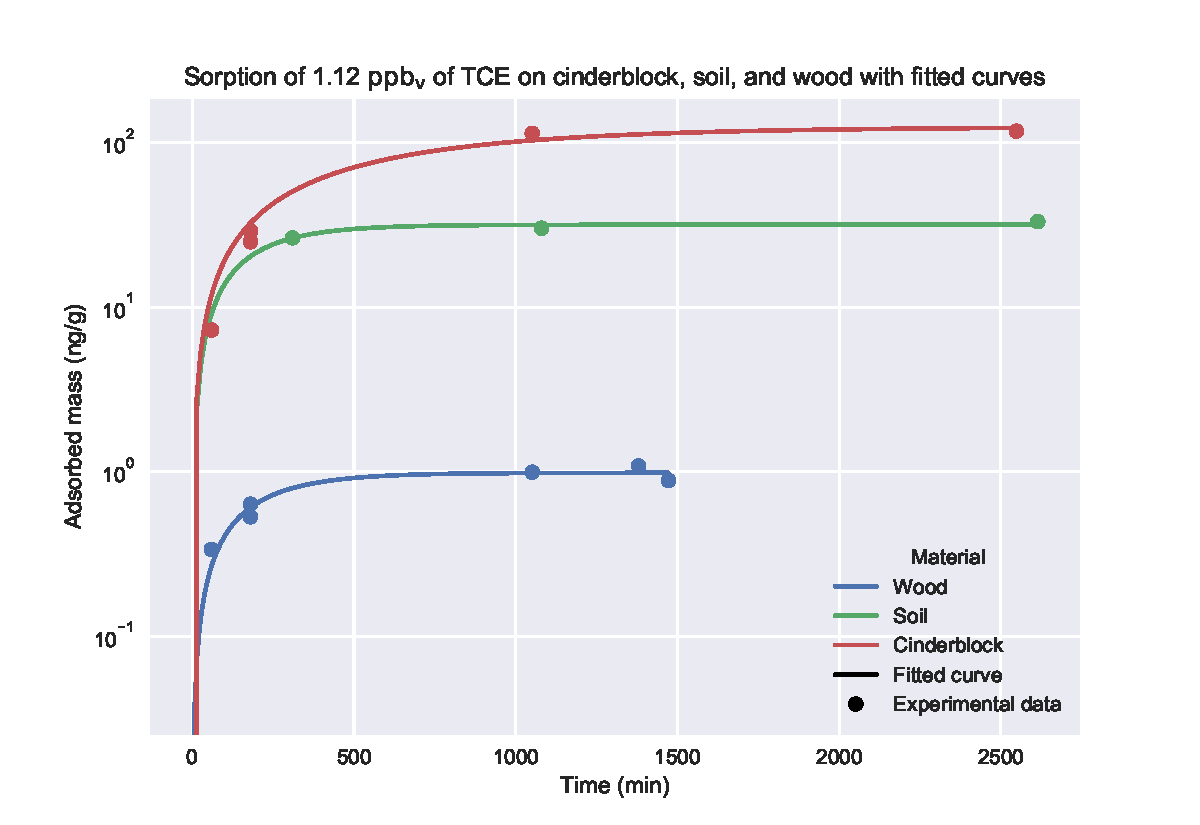
\includegraphics[width=\textwidth]{sorption_fit.pdf}
  \caption{Experimental data of sorption of TCE onto three select materials as well as fitted sorption rates based on the kinetic model \eqref{eq:sorption_rate}.}
  \label{fig:sorption_fit}
\end{figure}

% TODO: Shuai: Some thoughts or comments about these values? I.e. why is cinderblock so much larger?
Table \ref{tbl:sorption_fit} shows the fitted parameters for the tested materials.
Based on this these results we can see that cinderblock and soil have orders of magnitude larger sorption capacities than wood or drywall does.
We can also see by the $k_2$ values that soil and cinderblock sorb quickly, much faster than a material with similar sorptive capacity such as paper.
% Lots of "why is this?" here...

\begin{table}[htb!]
  \caption{Fitted kinetic sorption parameters based on sorption experiment data.}
  \label{tbl:sorption_fit}
  \centering
  \begin{tabular}{l c c c}
    \toprule
    Material & $k_1 \; \mathrm{(1/hr)}$ & $k_2 \; \mathrm{(1/hr)}$ & $K$ \\
    \hline
    Wood & 0.32 & 44.90 & $7.10 \cdot 10^{-3}$ \\
    Drywall & 0.41 & 87.94 & $4.65 \cdot 10^{-3}$ \\
    Carpet & 0.26 & 58.74 & $4.42 \cdot 10^{-3}$ \\
    Paper & 0.04 & 88.37 & $4.55 \cdot 10^{-4}$ \\
    Soil & 0.34 & 2636.57 & $1.30 \cdot 10^{-4}$ \\
    Cinderblock & 0.10 & 4175.16 & $2.40 \cdot 10^{-5}$ \\
    \bottomrule
  \end{tabular}
\end{table}



\subsection{Soil Sorption Retardation Effect}\label{sec:retardation_effect}

Building pressurization is a key factor in VI that influences the advective contaminant transport.
The magnitude of change in response to a pressurization change is significantly influenced by a range of factors, such as soil permeability, foundation depth, or soil moisture.
To demonstrate the effect that soil sorption has on contaminant soil mass transport in the VI context, we run two types transient simulation where initially the modeled structure is at a steady -5 Pa, i.e. slightly depressurized.
At the start of the simulation, the building building is 1) further depressurized to -15 Pa, or 2) overpressurized to 15 Pa, and the simulation is allowed to run for 72 hours.
\begin{align}
  \text{Depressurization}: \; \Delta p_\mathrm{in/out} &= \begin{cases}
    -5, \; &t = 0 \; \mathrm{(hr)} \\
    -15, \; &0 < t \leq 72 \; \mathrm{(hr)}
\end{cases}\\
\text{Overpressurzation}: \; \Delta p_\mathrm{in/out} &= \begin{cases}
  -5, \; &t = 0 \; \mathrm{(hr)} \\
  15, \; &0 < t \leq 72 \; \mathrm{(hr)}
\end{cases}
\end{align}
For each of these cases, the simulation is run using two different soil types - sand and sandy loam.
Sand is assumed here to not sorb any TCE, while for sandy loam a range of sorption isotherms are used.
These range from no sorption ($K_\mathrm{ads} = 0 \; \mathrm{(m^3/kg)}$) to the experimentally determined sorption isotherm ($K_\mathrm{ads} = 5.28 \; \mathrm{(m^3/kg)}$).\par
